\subsection{Анализ существующего приложения}

Первым шагом оптимизации является анализ исходного приложения, что включает в себя анализ структуры приложения, выявление связей между компонентами приложения а также функций, в которых происходит неэффективная обработка данных.

Структура приложения представлена на рисунке~\ref{img:oldStruct}.

\begin{figure}[H]
  \centering
  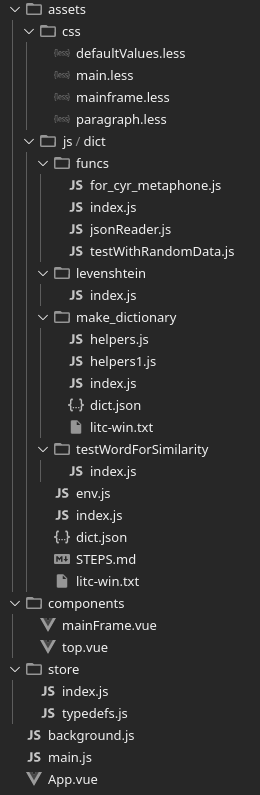
\includegraphics[height=0.4\textheight]{assets/images/practical/oldStructure.png}
  \caption{Структура исходного приложения}
  \label{img:oldStruct}
\end{figure}

При более детальном анализе кода приложения, было получено, что приложение состоит из двух частей: backend-часть, разработанная с использованием Electron и отвечающая за работу всего приложения, и front-end, разработанная с использованием Vue и отвечающая за визуальную составляющую приложения. Точкой входа в Electron-приложения является файл \emph{background.js}, а точка входа в Vue - \emph{main.js}.

В \emph{background.js} описано, какие настройки имеет окно приложения, какие настройки безопасности используются и по какому адресу расположен frontend, код представлен на рисунке~\ref{img:background_js}.


\begin{figure}[H]
  \centering
  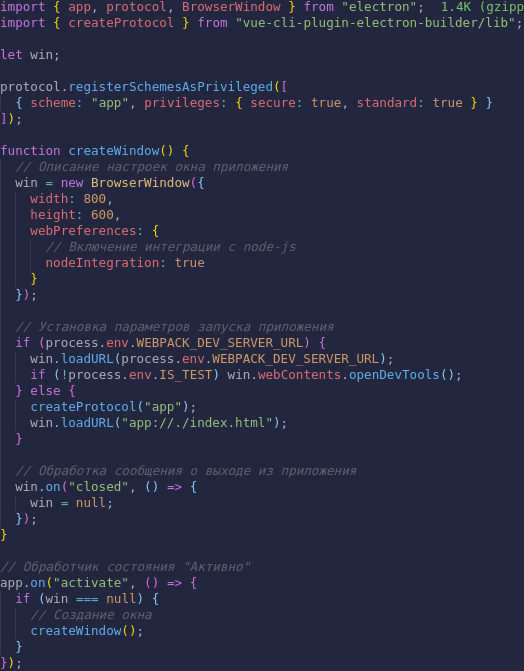
\includegraphics[height=0.4\textheight]{assets/images/practical/background_js.png}
  \caption{background.js}
  \label{img:background_js}
\end{figure}

В \emph{Vue} описано подключение к начальному HTML документу Vue-элементов, которые описаны в файле \emph{App.vue}, представляющем шаблон веб-приложения.

Vue-приложение использует плагин vuex для сохранения текущего состояния и обработки данных, при их изменении. В нём сохраняются текущие и предыдущие значения полей ввода. Свойство state Vue-хранилища представлено на рисунке~\ref{img:state}.

\begin{figure}[H]
  \centering
  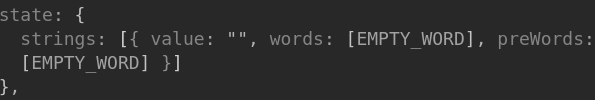
\includegraphics[width=0.95\textwidth]{assets/images/practical/state.png}
  \caption{Свойство state хранилища Vue}
  \label{img:state}
\end{figure}

Также здесь описаны методы получения и изменения состояния приложения.

В ходе анализа кода Vue-хранилища, было обнаружено несколько узких мест, укажу два из них.

Во первых, при загрузке элемента на страницу, вызывается действие getDict, которое вызывает функцию getDict, загружающую словарь, и, с интервалом в 4 секунды, производящую проверку слов в текущем поле ввода. Действия, производимые при загрузке страницы, приведены ны рисунках~\ref{img:mount},~\ref{img:getDict}.

\begin{figure}[H]
  \centering
  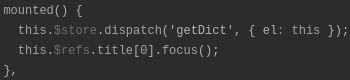
\includegraphics[height=0.1\textheight]{assets/images/practical/mounted.png}
  \caption{Загрузка элемента, 1}
  \label{img:mount}
\end{figure}

\begin{figure}[H]
  \centering
  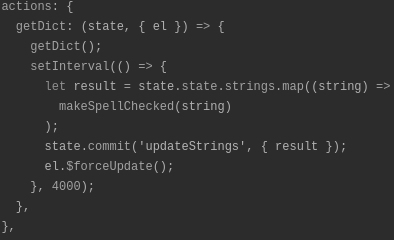
\includegraphics[width=0.5\textwidth]{assets/images/practical/getDict.png}
  \caption{Загрузка элемента, 2}
  \label{img:getDict}
\end{figure}

Такой метод вызова функции назначения глобальной переменной плох тем, что вызов произойдёт только после того, как компонент отобразится на странице приложения и некоторое время будет нельзя пользоваться переменной. Также здесь не оптимально вызывается функция проверки правописания - проверка происходит раз в 4 секунды для всех полей ввода. Это не целесообразно, так как пользователь мог ничего не вводить в течение этого времени пользователь мог ничего не ввести, но проверка всё равно запустится и произойдёт она для всех полей ввода, а не только для текущего.

Во вторых, загрузка словаря, по которому происходит проверка орфографии, находится в frontend и производится сторонним модулем. Код для загрузки представлен на рисунке~\ref{img:dictionary}.

\begin{figure}[H]
  \centering
  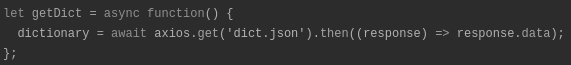
\includegraphics[width=0.95\textwidth]{assets/images/practical/dictionary.png}
  \caption{Загрузка словаря}
  \label{img:dictionary}
\end{figure}

Такой метод загрузки плох тем, что загрузка происходит не с помощью системных операций ввода-вывода, а с помощью методов обращения к внешним источникам, из-за чего процесс загрузки словаря занимает больше времени и увеличивает время загрузки приложения. Также здесь отсутствует обработка ошибок, возникающих при загрузке файла.

Также было выявлено использование копий одних и тех же данных в приложении и множество других узких мест.

По окончании анализа, было принято решение сменить фреймворк Vue на библиотеку React, ввиду того что Vue не покрывает все поставленные требования по производительности, и использовать другие способы загрузки словарей, отображения неправильно написанных слов, а так же использовать обособленный процесс, отвечающий за обработку слов.
